\chapter{Results}
\label{chap:Results}

Measured data for all experiment together with specification of computers used
for measure them is attached to this thesis. There we will discuss the results.

\section{Maximum edge weight experiment results}
\label{sec:results_maximum_edge_weight}

Experiment described in section \ref{sec:experiment_maximum_edge_weight} was
performed on both implementations and construction time and execution time of
operations were measured. Execution time per one operation is showed in the
following chart.

\begin{figure}[H]
\centering
\hsize=1.1\hsize
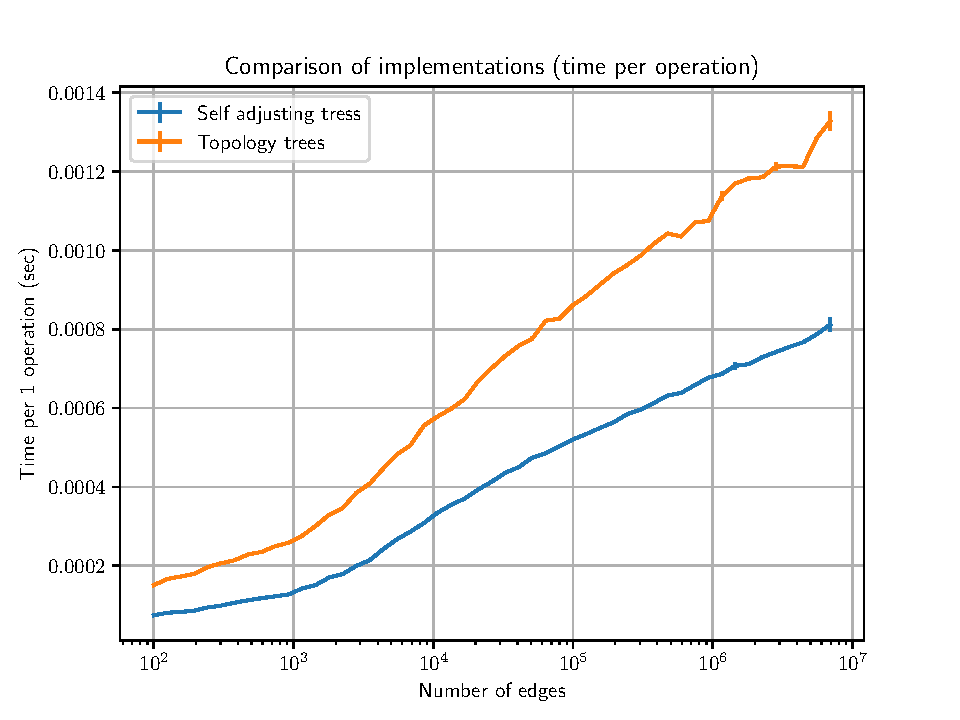
\includegraphics[width=\hsize]{charts/maximum_edge_weight_op.pdf}
\caption{Chart showing time per operation in the maximum edge weight experiment}
\end{figure}

Results show that both implementations have the same asymptotic time complexity
but as have been expected implementation with topology trees have larger
multiplicative constant.

Despite expectations this multiplicative constant is relatively small --
according to measured data the implementation with topology trees for larger
inputs (more than $10^4$ edges) is only $1.58$ to $1.68$ times slower than the
implementation which uses self adjusting trees.

\vfill\eject %% PRINTHACK

\subsubsection{Running time of construction}

Initial construction time measured per one edge of the initial underlying tree
is showed in the following figure. It shows some anomaly for small number of
edges (see bigger standard deviation in the beginning) but from tree size of
$10^4$ edges it stabilizes.

It shows that the implementation based on self adjusting trees could initialize
in approximately half time than the implementation based on topology trees,
which corresponds to time per operation in the previous chart.

\begin{figure}[H]
\centering
\hsize=1.1\hsize
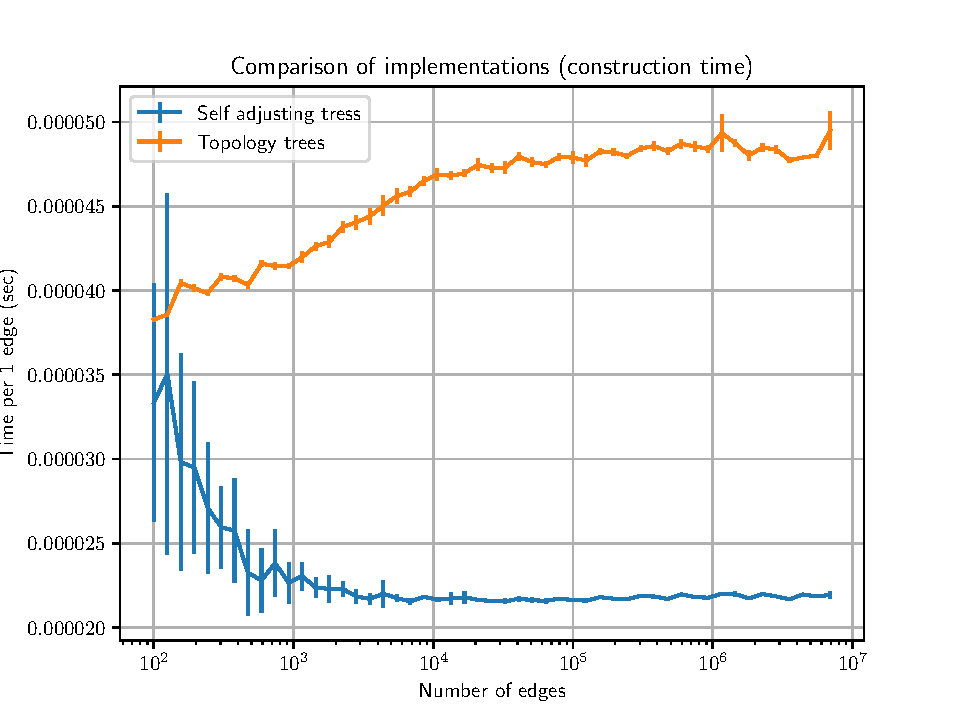
\includegraphics[width=\hsize]{charts/maximum_edge_weight_construction.pdf}
\caption{Chart showing construction time per one edge in the maximum edge weight
experiment}
\end{figure}

\vfill\eject %% PRINTHACK

\section{Edge 2-connectivity experiment results}
\label{sec:results_edge_2_connectivity}

Similarly to the previous experiment the experiment described in the section
\ref{sec:experiment_edge_2_connectivity} was performed on both implementations
(on second with normal updates and with expensive updates turned off during
query). Construction time (time to insert all initial edges) and execution time
of all operations and execution time on only query operations were measured.

\subsubsection{Running time of all operations}

Firstly analyze the running time of normal operations. As you can see on the
following chart, all implementations have the same asymptotic complexity (they
should operate in $\O(\log^4 N)$). The implementation which uses self adjusting
trees has the lowest multiplicative constant as have been expected.

\begin{figure}[H]
\centering
\hsize=1.1\hsize
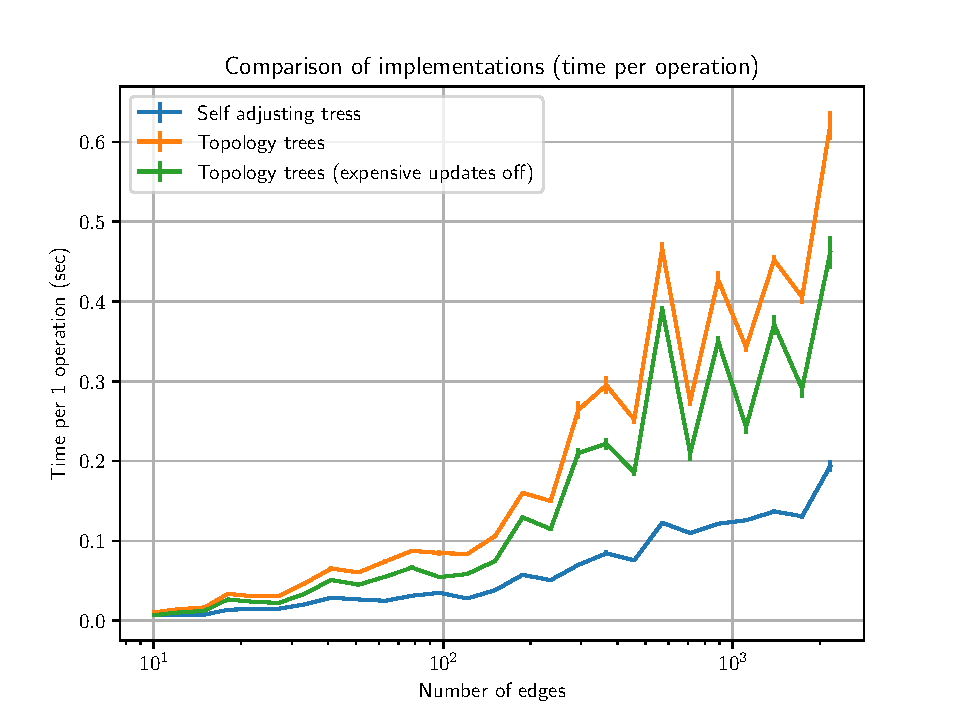
\includegraphics[width=\hsize]{charts/double_edge_connectivity_op.pdf}
\caption{Chart showing time per any operation in the edge 2-connectivity experiment}
\end{figure}

The implementation with topology trees is $2.2$ to $3.5$ times slower than the
implementation which uses self adjusting trees. This multiplicative constant is
larger than the same multiplicative constant in the first experiment.

Mark multiplicative constant from the experiment
\ref{sec:results_maximum_edge_weight} as $C$. Expected value for the
multiplicative constant in this experiment would be $C^3$ (because operations in
this experiment have asymptotic time complexity of $\O(\log^3 N)$ or $\O(\log^4
N)$), but measured multiplicative constant for this experiment is lower. The
difference against the expectation is probably caused by processor caches --
updates in the edge 2-connectivity experiment operates on arrays in the clusters
in sequential order and this cause less cache misses.

Another interesting observation is that turning of expensive updates during
queries have lowers the running time only about 30 \% although the ratio of
queries was 70 \% in all the experiments -- so the most time is spent in the
insertions and deletions of edges.

\subsubsection{Running time of only queries}

In some uses there might be crucial to quickly answer on queries and other
updates may be slower. The second experiment executed only queries and measured
their running time.

\begin{figure}[H]
\centering
\hsize=1.1\hsize
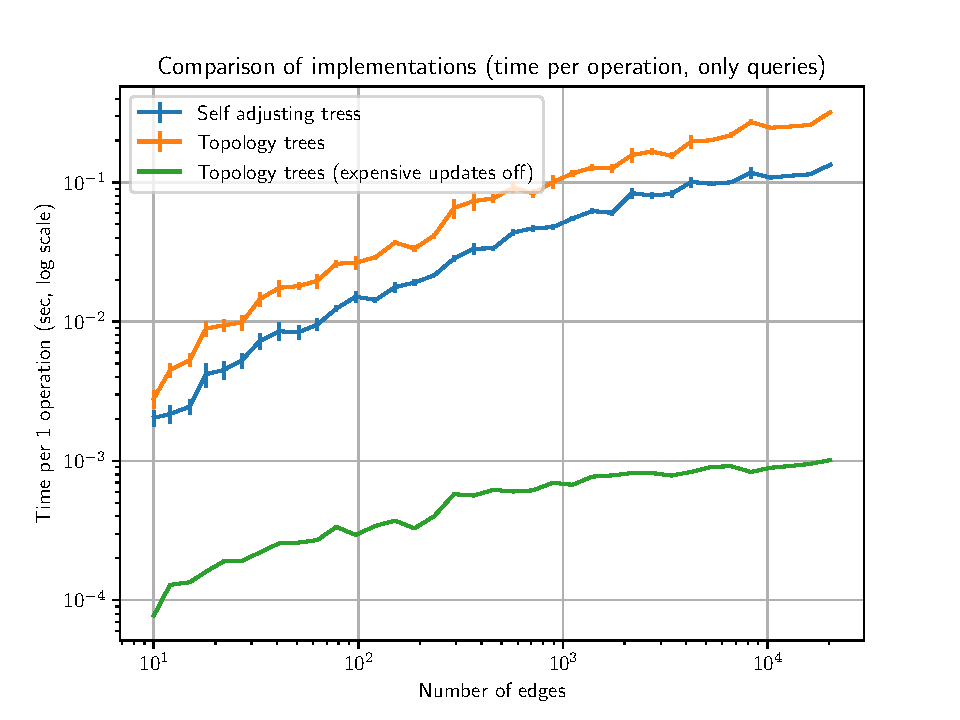
\includegraphics[width=\hsize]{charts/double_edge_connectivity_op_queries.pdf}
\caption{Chart showing time per query in the edge 2-connectivity experiment}
\end{figure}

As you can see on the above chart (it has logarithmic scale on the time axis)
the implementation where we could turn off expensive updates during query --
topology trees implementations -- is the absolute winner. Time complexity of
the implementation without expensive updates is asymptotically lower than the
time complexity of any other implementation.

\subsubsection{Running time of construction}

Construction in this problem cannot be done in one step from some underlying
tree, but it has to be done by sequentially inserting all the edges from the
underlying graph. Thus time of construction of graph with $M$ edges is time of
sequential insertion of $M$ edges into the empty structure.

\begin{figure}[H]
\centering
\hsize=1.1\hsize
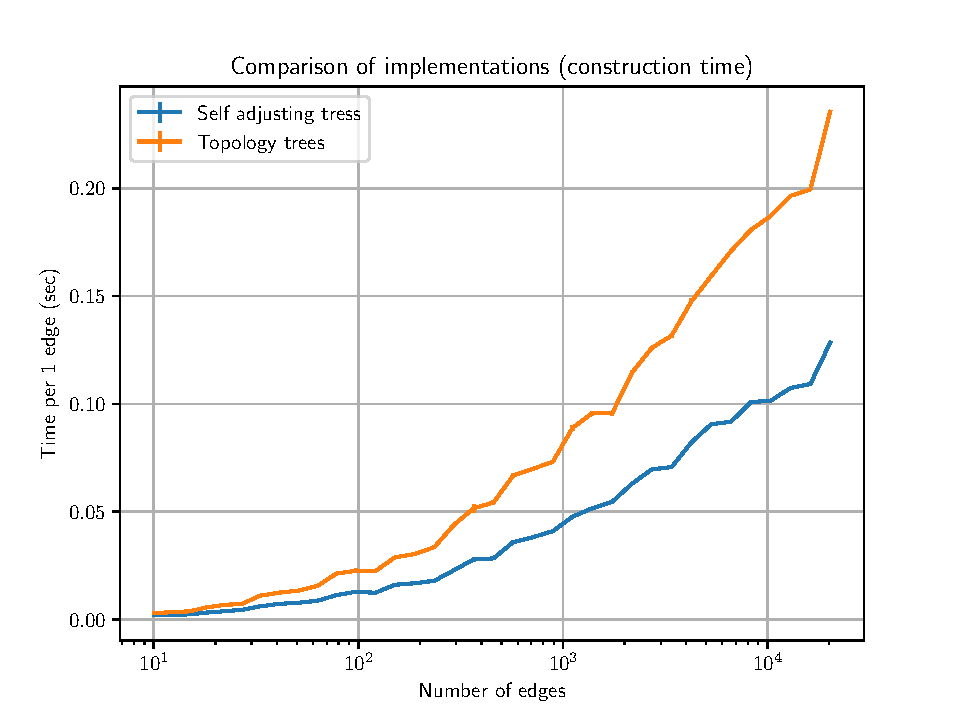
\includegraphics[width=\hsize]{charts/double_edge_connectivity_construction.pdf}
\caption[Chart of construction time per edge in the edge 2-connectivity experiment]
{Chart showing construction time per one edge in the edge 2-connectivity experiment}
\end{figure}

As you can see the construction time is similar and as have been expected the
implementation which uses topology trees is slower. According to measurement
it is $1.7$ to $1.9$ times slower than the construction of the implementation
which uses self adjusting trees.

Not so good result is that the construction time per one edge grows with the
graph size and from some size it starts to be unsuitable for real use. For
production use it would need some construction method like the maximum edge
weight problem.
